\chapter{Relevante Grundlagen und Überblick über alternative Antriebe}
\label{ch:Relevante Grundlagen und Überblick über alternative Antriebe}
Für die Analyse der Forschungsfrage es ist wichtig die zentralen theoretischen Begriffe zu definieren. 
Das Kapitel \ref{s:Bodenabfertigung eines Luftfahrzeugs} stellt die Grundlagen der Flugzeugabfertigung und Definition
der beteiligten Stakeholder am Flughafen dar. Zunächst beschäftigt sich das Kapitel \ref{s:Kosten}
mit bedeutenden Informationen zu Kosten am Flughafen, gefolgt von Emission-Regulierungsinitiativen im Kapitel \ref{s:Klimapolitische Maßnahmen}. 
Anschließend werden im Teil \ref{s:Neuartige Antriebe}
die neuartigen alternativen Antriebe und Konzepte und Flugzeugmodelle mit diesen Antrieben vorgestellt.

\section{Stakeholder am Flughafen}
\label{s:Stakeholder am Flughafen}
%
\begin{figure}[h]
	\centering
	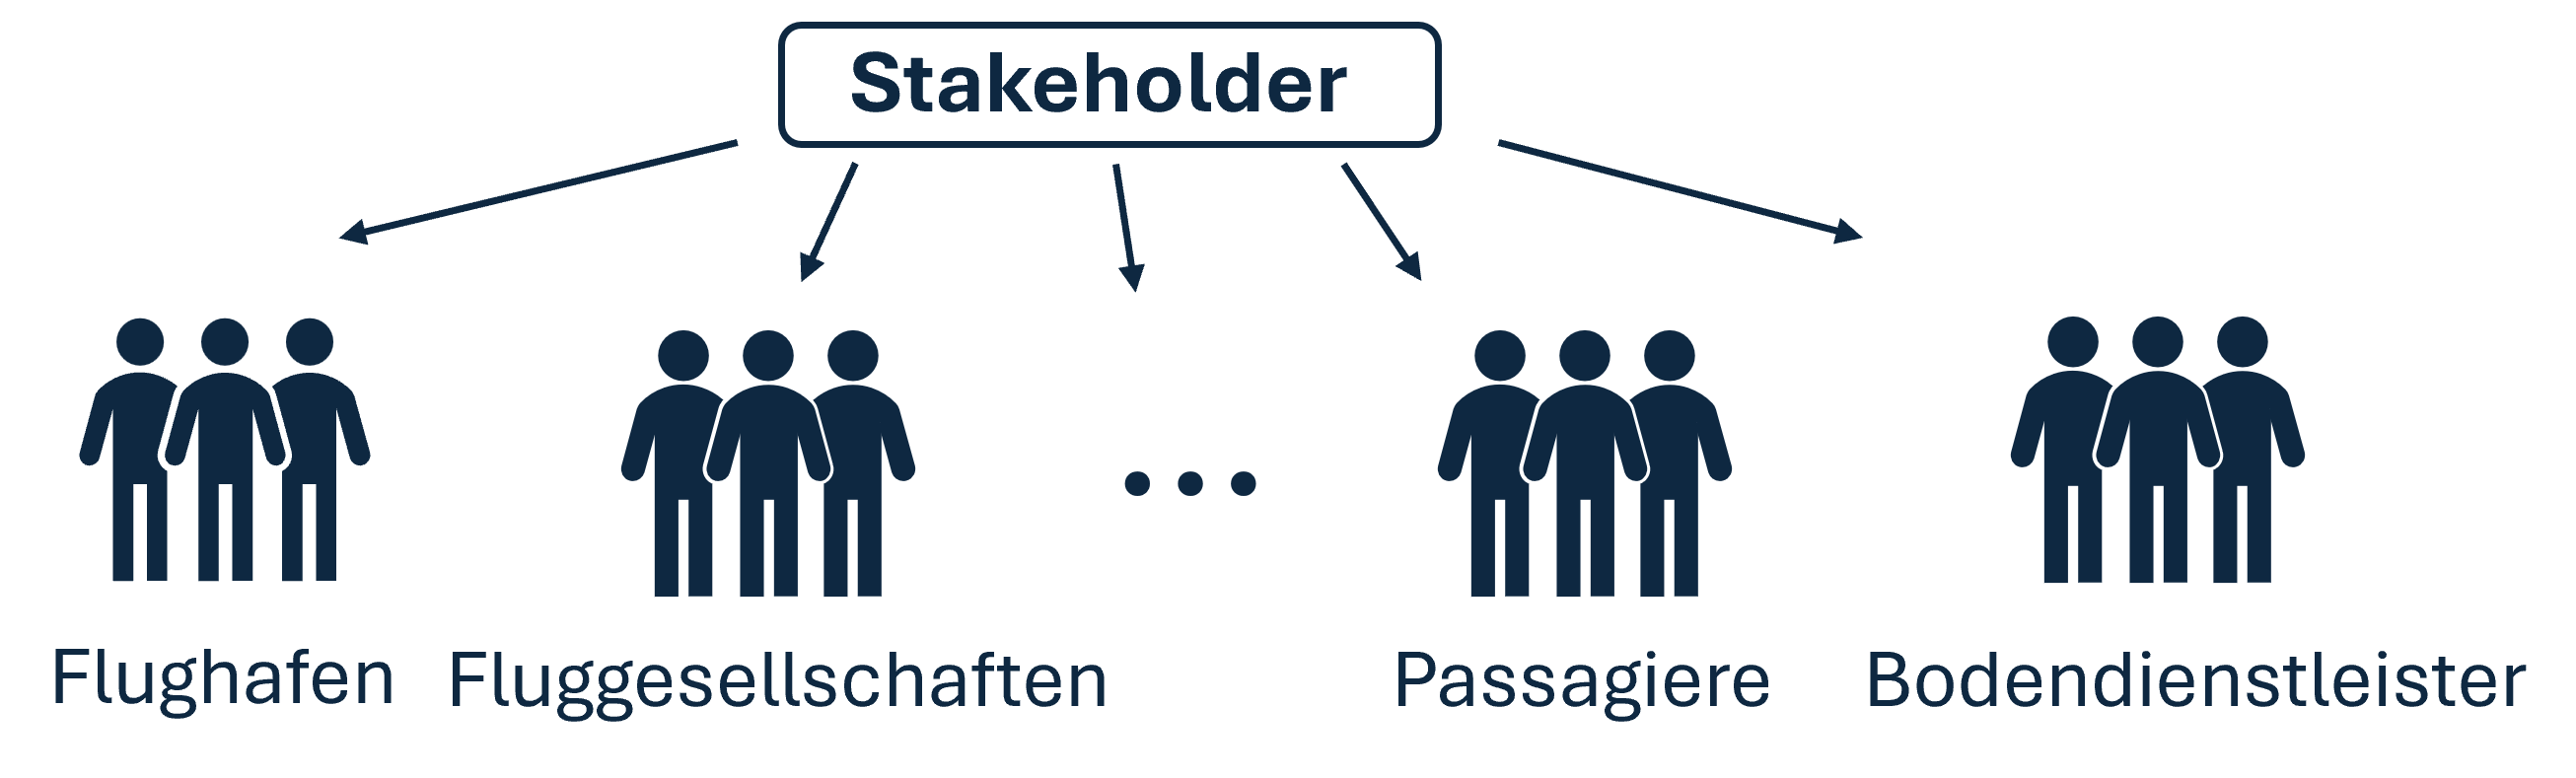
\includegraphics[width=0.8\linewidth]{Bilder/Stakeholder.png}
	\caption[Relevante Stakeholder am Flughafen]{Relevante Stakeholder am Flughafen}
	\label{stakeholder}
\end{figure}

Am Flughafen ist eine Vielzahl an Stakeholdern beschäftigt, die miteinander agieren. 
Durch die neuen Luftfahrzeugantriebe steht diesen Akteuren eine schwierige Aufgabe bevor. 
Gute Zusammenarbeit der Stakeholder fördert die Pünktlichkeit der Abfertigung und 
hilft Verspätungen zu vermeiden \cite{schmidt2016challenges}.

\subsubsection{Flughafenbetreiber}
Einer der Stakeholder am Flughafen ist der Flughafenbetreiber selbst. 
Der Flughafen stellt die Fluggerät- und Passagierabfertigungs-Infrastruktur wie bspw. 
Terminals oder Start- und Landebahnen zur Verfügung (welche als Kernfunktionen gelten), 
wofür Nutzungsgebühren erhoben werden \cite{conrady2019luftverkehr}. %Seite 180, falls ich Entgelte durchzählen will.

Zum Flughafen gehören außer Start- und Landebahnen unter anderem 
Rollwege, Vorfeld, sowie die Infrastruktur für Gepäckabfertigung. 
Größere Flughäfen verfügen über eine Tankfarm am Flughafenstandort. 
Zu dieser Tankfarm gehören mehrere Anlagen, die mit der Betankung verbunden sind, darunter Treibstofftanks \cite{moriarty2024sustainable}.
Darüber hinaus stellen Flughäfen eine intermodale Verknüpfung dar \cite{conrady2019luftverkehr}. %d.h. die Anbindung an anderen Verkehrsmitteln wird hergestellt.
Direkte Nutzer von Flughäfen sind Im- und Exporteure von Dienstleistungen und Waren \cite{schaar2010analysis}. 

Flughäfen sind ein großer Teil der regionalen Wirtschaft \cite{schaar2010analysis} 
und sorgen für eine Vielzahl von Arbeitsstellen. 
Andererseits verursachen sie ein Ausmaß an Lärm und Umweltbelastungen, 
welche durch die Emissionen der Flugzeuge entstehen.
Zur Kompensation verlangt der Flughafen hierfür ebenfalls Entgelte. %Kap 4

Für die Entwicklung der Infrastruktur und Begleichung der Betriebskosten müssen Flughäfen 
gelegentlich finanzielle Unterstützung aus anderen Quellen, wie staatlicher Subventionen, 
in Anspruch nehmen \cite{schaar2010analysis}. 

Flughäfen in Deutschland sind überwiegend in öffentlicher Hand \cite{conrady2019luftverkehr}.
Die Europäische Kommission besagt, dass Flughäfen mit einem Passagieraufkommen von über 3 Millionen 
Passagiere jährlich in der Lage sind, ihre Betriebskosten selbst durch Gewinn zu decken.
\footnote{\glqq Leitlinien für staatliche Beihilfe für Flughäfen und Luftverkehrsgesellschaften\grqq{} 2014/C 99/03}
%Und die kleineren Flughäfen durch weniger Betrieb mehr auf die Hilfe angewiesen.
Eine Kategorisierung der Flughäfen basiert auf der Passagiermenge. 
Der Europäischen Kommission nach werden die Flughäfen nach jährlichem Passagieraufkommen folgend unterteilt: 
\begin{itemize}
    \item große Gemeinschaftsflughäfen > 10 Mio. Passagieren;
    \item nationale Flughäfen mit 5 bis 10 Mio. Passagieren;
    \item große Regionalflughäfen mit 1 bis 5 Mio. Passagieren;
    \item kleine Regionalflughäfen < 1 Mio. Passagieren.
\end{itemize}
Aufgrund dieser Kategorisierung in dem Jahr 2023 gab es in Deutschland 
sieben große Gemeinschaftsflughäfen, einschließlich zwei Hubs, und 16 Regionalflughäfen \cite{Destatis_Luftverkehr_2024}.
Ein Hub zeichnet sich durch einen großen Flughafen mit hohem Anteil an Umsteigeverkehr aus.

\subsubsection{Fluggesellschaft}
Fluggesellschaften sind Dienstleister, welche die Infrastruktur eines Flughafens für die 
Abfertigung von Passagieren und Fracht nutzen. 
Sie sind gewinnorientiert und haben das Ziel wettbewerbsfähig zu bleiben. 
Für eine Fluggesellschaft ist von Relevanz, wie hoch die Beträge
sind, die der Flughafen verlangt \cite{schaar2010analysis}. 
Die Beträge unterscheiden sich sowohl je nach Flughafengröße und -strategie, als auch im Flugzeugtyp.

%Fluggesellschaften und Treibstoff-Firmen sind für die sichere Betankung verantwortlich. Quelle: Annex 14 (Doc 9137 Teil 8)
\subsubsection{Bodenverkehrsdienste} %S. 183 conrady
%
Bodenverkehrsdienste sind für die Abfertigung der Flugzeuge auf dem Boden zuständig.
Nach Conrady \cite{conrady2019luftverkehr} gehört zu ihren Tätigkeiten außerdem:  
die Fluggastabfertigung, administrative Abfertigung sowie Transportdienste von Fracht, Post und Gepäck bis zum Flugzeug \cite{mensen2013handbuch}.
Sie sind auf Infrastruktureinrichtungen wie Gepäckförderanlagen und Betankungsanlagen 
sowie weitere Grundausstattung am Vorfeld angewiesen. 
Die Abfertigung kann entweder von einer Fluggesellschaft, einem Flughafen oder einem 
unabhängigen Dienstleister durchgeführt werden. 
Meistens werden die Bodenverkehrsdienste in Deutschland von den Flughäfen übernommen.\\ %oder die externen Firmen (Dritte) werden engagiert.
%
Zu weiteren Vorfelddiensten gehören Betankungs-, Reinigungsdienste und Wartungsdienste.
Wartungsdienste führen die routinemäßige Kontrolle der Flugzeuge vor den Flügen durch.
Reinigungsdienste und der Flugzeugservice sind für die Reinigung eines Flugzeugs 
von Innen und Außen, Wasserservice, die Klimaanlagen in der Kabine und die Enteisung verantwortlich.
%Betankungsdienste führen nicht nur die Be- und Entladung sowie Lagerung durch, 
%sie sind sondern auch für andere Flüssigkeiten (wie z.B. Öl) zuständig.
%
%
%OPS 1.1150 "Handling agent. An agency which performs on behalf of the operator some or all of the latter's functions
%including receiving, loading, unloading, transferring or other processing of passengers or cargo;"
%
%Von der Fluggesellschaft werden Handling Agents eingestellt, der die ganze Abfertigung und Kommunikation zwischen Beteiligten am Vorfeld
%kontrollieren.
%In dieser Arbeit werden nur die internationale und regionale Verkehrsflughäfen betrachtet. 
%(Es bietet sonstige Serviceleistungen für die Passagiere, wie Parkplätze, Handel Dienstleistungen.)
%
Zu den Stakeholdern am Flughafen zählen ebenfalls Luftfahrzeughersteller, Flugsicherungen, 
Reiseveranstalter, staatliche Institutionen \cite{maertens2023neue},
sowie Beteiligte wie Passagiere und Arbeitskräfte. 
Sie nehmen nicht direkt an der Flugzeugabfertigung bzw. am Betrieb am Vorfeld teil, 
deswegen stehen sie nicht im Fokus dieser Arbeit.
Analog hierzu wird die Flugsicherung aufgrund unveränderter Umstände
durch alternative Antriebe nicht betrachtet. 
Die Arbeit wird sich auf die Betriebskosten einer Fluggesellschaft 
und Infrastrukturkosten des Flughafens fokussieren.
%
%Auf die Kosten eingehen:
%Laut OPS 1.175 %"The number of ground staff is dependent upon the nature and the scale of operations"
%Anzahl der benötigten Bodenmitarbeiter ist von dem Maßstab der Operationen am Flughafen anhängig.
%
%BAs können weniger überlastete Flughäfen anfliegen und entferne Bereiche, und
%nur die geringe Bedarf abdecken.
%Europäische Kommission Leitlinien für staatliche Beihilfe für Flughäfen und Luftverkehrsgesellschaften 2014/C 99/03
%
%Als Regionalflughafen definiert E Kommissionen einen Flughafen mit bis zu 3 Millionen Passagieren im Jahr.
%Flughäfen mit mehr als eine Million Passagieren im Jahr decken überwiegend ihre Betriebskosten selbst. %egal?
%
%„Betriebskosten“: die mit der Erbringung von Flughafendienstleistungen verbundenen Kosten eines Flughafens;
% dazu gehören Kostenkategorien wie Personalkosten, Kosten für fremdvergebene Dienstleistungen, Kommunikation, 
% Abfallentsorgung, Energie, Instandhaltung, Mieten und Verwaltung, jedoch weder Kapitalkosten, Marketingunterstützung 
% bzw. andere Anreize, die der Flughafen den Luftverkehrsgesellschaften bietet, noch Kosten für Aufgaben mit hoheitlichem Bezug;
%
%
%Der Bedarf an öffentlichen Mitteln zur Betriebskostenfinanzierung variiert unter den derzeitigen Marktbedingungen
% aufgrund der hohen Fixkosten in der Regel je nach Flughafengröße und ist normalerweise bei kleineren Flughäfen
% verhältnismäßig höher. Unter den derzeitigen Marktbedingungen können nach Auffassung der Kommission in Bezug auf
%   die jeweilige finanzielle Tragfähigkeit nachstehende Kategorien von Flughäfen abgegrenzt werden:
%
%d)Flughäfen mit 1 bis 3 Millionen Passagieren im Jahr dürften im Durchschnitt in der Lage sein, ihre Betriebskosten überwiegend selbst zu tragen;
%
%e)Flughäfen mit mehr als 3 Millionen Passagieren im Jahr erzielen in der Regel einen Betriebsgewinn und dürften 
%in der Lage sein, ihre Betriebskosten zu decken.
\section{Bodenabfertigung eines Luftfahrzeugs}
\label{s:Bodenabfertigung eines Luftfahrzeugs}

Zur Veranschaulichung der Änderungen an der Infrastruktur am Flughafen, 
welche durch neuartige Antriebe vorgenommen werden müssen, ist es notwendig 
wichtige Begriffe einer Abfertigung des konventionellen Flugzeugs hervorzuheben. 
Unter konventionellen Luftfahrzeugen sind die zu verstehen,
die mit fossilen Treibstoffen, wie erdölbasiertes Kerosin, betrieben werden. 
Der Fokus wird auf die gewerblichen Passagierflugzeuge gelegt,
da sie einen erheblichen Teil an zivile Luftverkehr ausmachen. %%%%%% ZAHL FINDEN

Die Blockzeit setzt sich aus der Zeit vom Beginn der Bewegung von der Parkposition 
bis zum Ende der Bewegung zur Parkposition, einschließlich der Flugzeit, zusammen.
An der Parkposition des Flughafens werden die Triebwerke ausgeschaltet 
und der Ablauf eines Turnarounds beginnt. 
Mensen \cite{mensen2013handbuch} definiert den Turnaround, 
wie die Abfertigung der Flüge, die zeitnah zusammen liegen. % satz komisch
Bei einem Turnaround wird das Luftfahrzeug durch viele Akteure am Flughafen, 
wie Flugplatzbetreiber, Fluggesellschaft und Dritte, für den nächsten Flug vorbereitet. 
Es muss ausgeladen, kontrolliert, gereinigt, anschließend mit Treibstoff und Wasser versorgt %%%%%%%% HINZUFÜGEN
und für den nächsten Flug beladen werden.\\

Die Abbildung \ref{abfertigung} stellt die Abfertigung eines Flugzeugs an der Parkposition dar.
Nach ICAO Doc 9157 besteht Abfertigung eines Passagierflugzeugs 
insgesamt aus Passagier-, Gepäck- und Frachtabfertigung, Sanitärservice, Wasserbetankung, 
Gepäckabfertigung, Betankung, Stromversorgung, Startluft, Flugzeugschleppen, 
Bordküchenservice, Wartungsservice sowie Bereitstellung einer Klimaanlage und Sauerstoff,
wie in der Abbildung dargestellt. Durch neuartige Antriebe kann es aufgrund anderer 
technischer Grundlagen zu Änderungen in diesen Prozessen kommen.
%
Der Betankungsvorgang ist ein wesentlicher Teil der Flugzeugabfertigung. 
Zurzeit werden für Lufttransport die Treibstoffe auf Basis fossiler Stoffe, wie Erdöl, genutzt. 
Laut EU-OPS 1.305 darf das Luftfahrzeug aus Sicherheitsgründen erst mit dem konventionellen Treibstoff betankt werden, 
wenn sich keine Passagiere an Bord befinden. 
%
%Das Flugzeug wird an ein Hilfstriebwerk (auxiliary power unit - APU) angeschlossen \cite{mensen2013handbuch}. 
%Die APU liefert Strom, wenn die Haupttriebwerke nicht laufen (quelle: [Annex 14. Doc 9137 Part 8]).
%Parallel werden Fracht und sonstige Gepäckeinheiten mit dem Hubwagen abgeladen und mit Transporthängern zur Sortieranlage 
%im Terminal gebracht \cite{mensen2013handbuch}. Im Falle, das die Parkposition direkt am Flughafen ist, 
%können Passagiere direkt über die Treppe oder Fluggastbrücke zum Terminalgebäude gelangen. 
%Wenn die Parkposition am Vorfeld liegt, muss auf einen Bus zurückgegriffen werden. 

\begin{figure}[h]
	\centering
	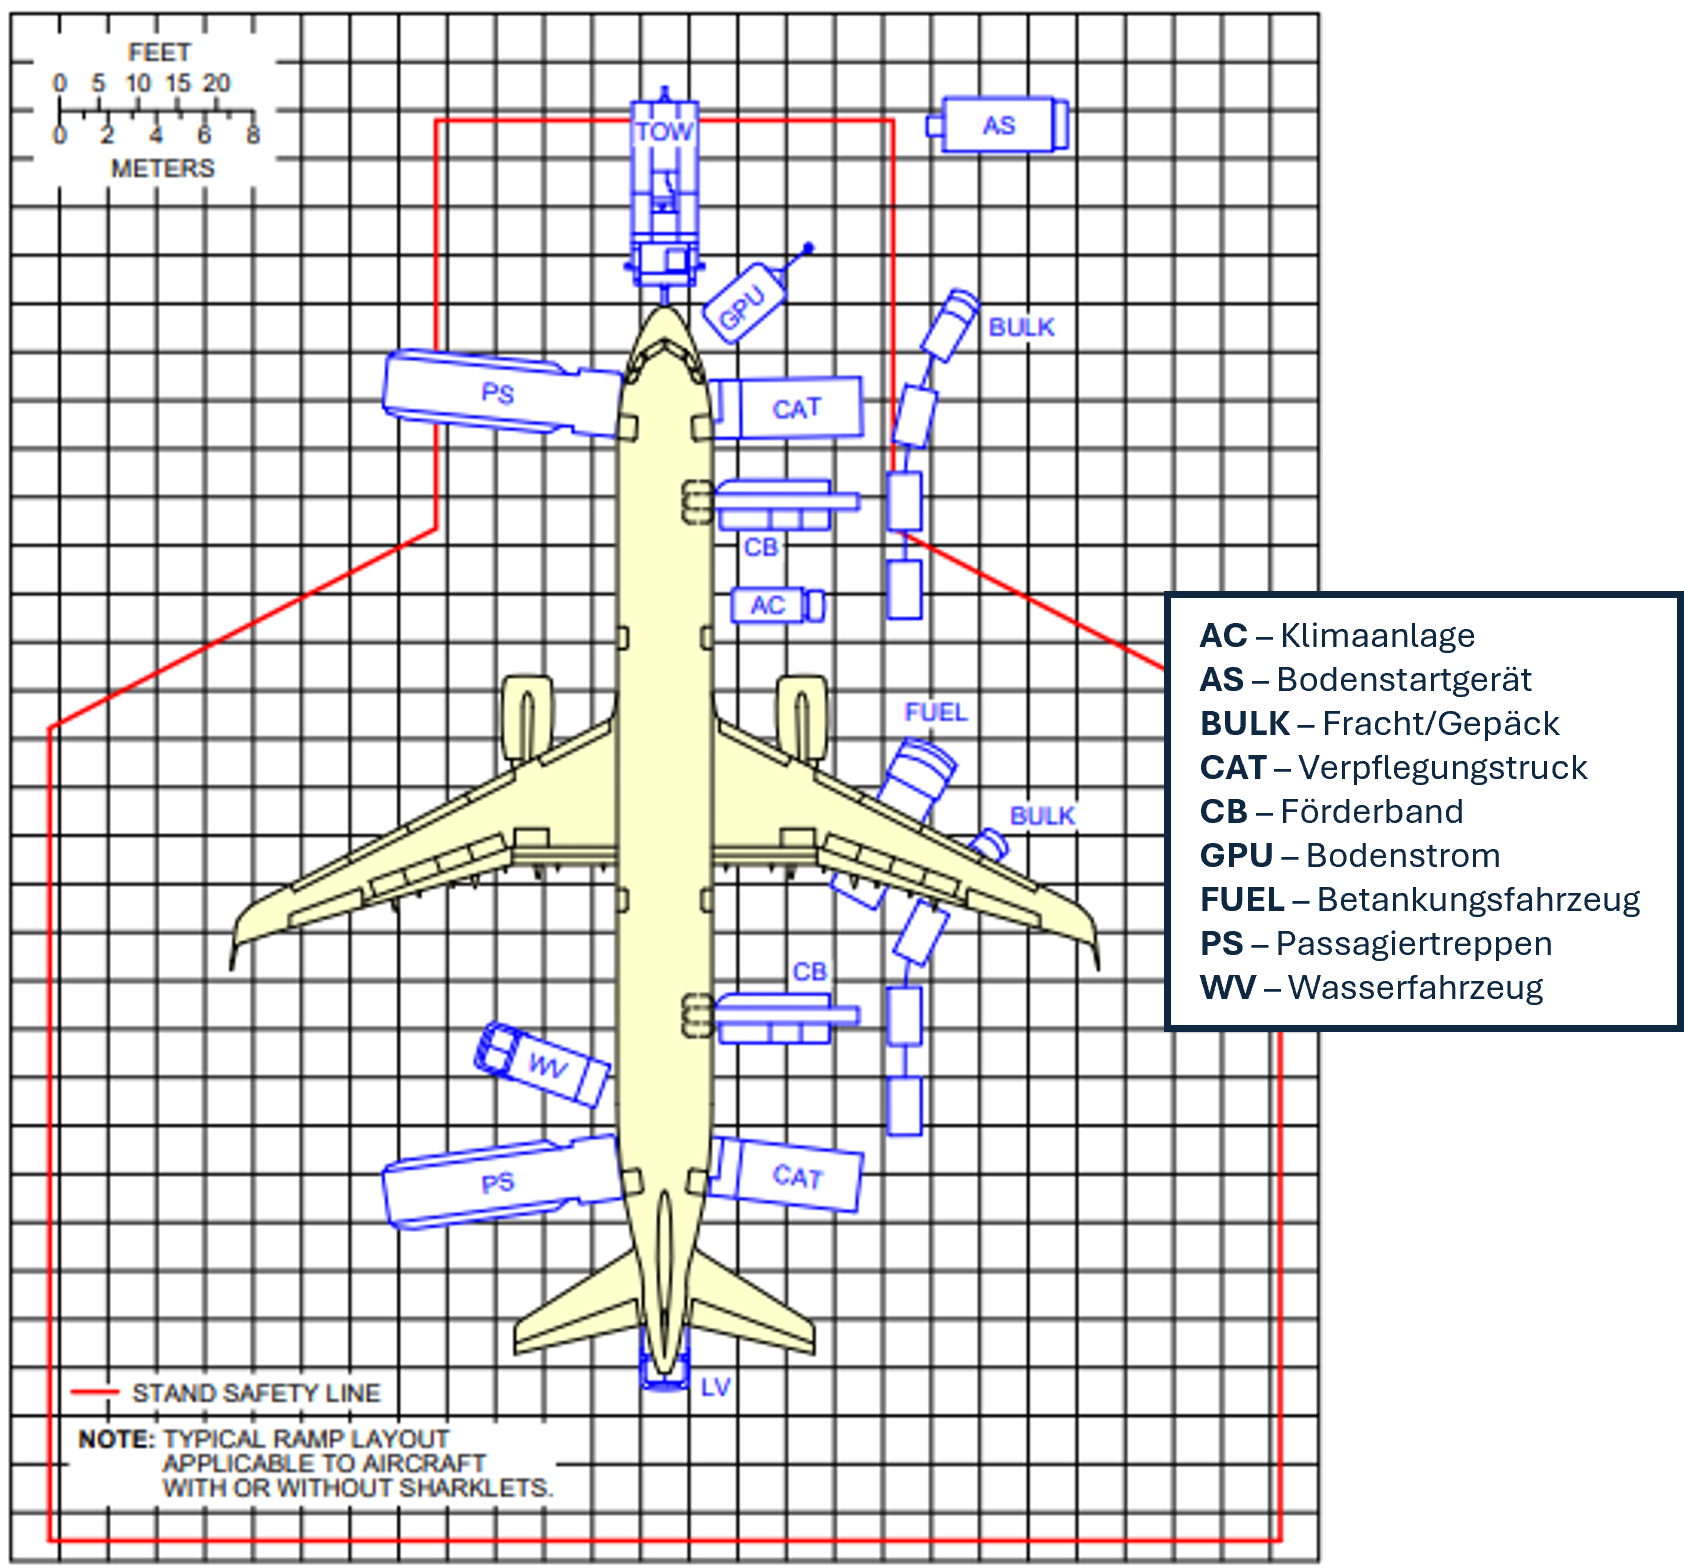
\includegraphics[width=0.8\linewidth]{Bilder/A321_Abfertigung.png}
	\caption[Abfertigung eines Flugzeugs am Parkposition]{Abfertigung eines A321 \cite{airbus2022a321} mit eigenem Hinweis}
	\label{abfertigung}
\end{figure}

Je nach Flugdistanz und Flugzeuggröße kann es zu unterschiedlichen Abfertigungszeiten führen. 
Bei kleineren Flugzeugen ist die Abfertigungszeit kürzer, als die eines größeren Luftfahrzeuges. 
In Bezug auf die Transportdistanz wird nach Kurz- (ca. 2 Stunden oder bis 1000 km) 
und Mittelstreckenflügen (bis 3,5 Stunden oder bis 3000 km) und 
Langstreckenflügen (ab 3,5 Stunden und ab 3000 km) unterschieden \cite{mensen2013handbuch}.
Die Definition von Distanzen variiert teils erheblich, 
z.B. definiert der Flughafen Frankfurt Langstrecken ab 6000 km.% diese Werte werden auch im Kapitel \ref{s:Betriebsszenarien} genutzt.

%Die Preise für fossilen Energie sind durch wirtschaftlichen Umgebung geprägt, wo

%whereas biofuels produced at stand-alone facilities are
%moved by rail or barge/tanker (large volumes) or truck (small volumes)
%https://www.osti.gov/servlets/purl/2440801
%A tank farm
%comprises multiple interconnected pieces of equipment designed to safely receive, store, and
%dispense fuel to a hydrant system or truck delivery to aircraft. Although not an all-inclusive list, a
%tank farm consists of tanks; pipeline interconnection; equipment to control the flow of fuel and
%vapors; meters to measure the volume of fuels into the tank farm and out to aircraft; filters to
%remove contaminants; pumps to move fuel throughout the system; safety equipment to prevent,
%detect, and contain leaks throughout the system; off-loading racks to fill fuel trucks; and hydrant
%systems—underground pipes and hydrants
Größere Flughäfen haben eine Tank Farm am Flughafenstandort. Zur dieser Tankfarm gehören mehrere mit Anlagen, die mit
der Betankung verbunden sind, ein davon sind Treibstofftanks.
